% THIS IS AN EXAMPLE DOCUMENT FOR VLDB 2012
% based on ACM SIGPROC-SP.TEX VERSION 2.7
% Modified by  Gerald Weber <gerald@cs.auckland.ac.nz>
% Removed the requirement to include *bbl file in here. (AhmetSacan, Sep2012)
% Fixed the equation on page 3 to prevent line overflow. (AhmetSacan, Sep2012)

\documentclass{vldb}
\usepackage{times, graphicx, url, xcolor, multicol, minipage, subfig, tikz, draftwatermarkbottom, draftwatermarktop}
\usepackage{balance}  % for  \balance command ON LAST PAGE  (only there!)

\renewcommand{\ttdefault}{fi4}

\usetikzlibrary{positioning, snakes, shapes}

\newenvironment{myitemize}
{

   \vspace{0mm}
    \begin{list}{$\bullet$}{\leftmargin=1em}
        \setlength{\topsep}{0em}
        \setlength{\parskip}{0pt}
        \setlength{\partopsep}{0pt}
        \setlength{\parsep}{0pt}         
        \setlength{\itemsep}{.25em} 
        \setlength{\itemindent}{0em}
}
{
    \end{list} 
    \vspace{-.5em}
}

\newenvironment{myenumerate}
{

   \vspace{0mm}
   \newcounter{qcounter}
    \begin{list}{\arabic{qcounter}.~}{\usecounter{qcounter}\leftmargin=1em}
        \setlength{\topsep}{0em}
        \setlength{\parskip}{0pt}
        \setlength{\partopsep}{0pt}
        \setlength{\parsep}{0pt}         
        \setlength{\itemsep}{.25em} 
        \setlength{\itemindent}{0em}
}
{
    \end{list} 
    \vspace{-.5em}
}

\begin{document}


% ****************** TITLE ****************************************

\title{Highly Available Transactions: Virtues and Limitations}
{\author{Peter Bailis{\fontsize{12}{14}$^\dagger$}, Aaron Davidson{\fontsize{12}{14}$^\dagger$}, Alan Fekete{\fontsize{12}{14}$^\diamond$}, Ali Ghodsi{\fontsize{12}{14}$^{\dagger,\ddagger}$}, Joseph M. Hellerstein{\fontsize{12}{14}$^\dagger$}, Ion Stoica{\fontsize{12}{14}$^\dagger$}\\{{\fontsize{12}{14}$^\dagger$}\hspace{.5mm}UC Berkeley\hspace{4mm}{\fontsize{12}{14}$^\diamond$}\hspace{.5mm}University of Sydney\hspace{4mm}{\fontsize{12}{14}$^\ddagger$}\hspace{.5mm}KTH/Royal Institute of Technology}}}
\maketitle

\begin{abstract}
To minimize network latency and handle the possibility of partial
failure and network partitions, many modern distributed systems eschew
transactional functionality, which provides strong semantic guarantees
for groups of multiple operations over multiple data items. In this
work, we consider the problem of achieving transactional guarantees
with high availability, or without suffering from unavailability
during system partitions or incurring high network latency.  We
introduce a new taxonomy of high availability and analyze a
combination of ACID and distributed consistency guarantees to identify
which can and cannot be achieved by Highly Available Transaction (HAT)
systems. In doing so, we analytically and experimentally quantify the
benefit of providing high availability as well as the associated
semantic compromises.
\end{abstract}



\section{Introduction}

Many recent systems have eschewed ACID guarantees.

CAP Theorem says you can't have consistency and availability and also talks about partitions.

What does CAP have to say about ACID? Recent workshop result on Highly Available Transactions briefly demonstrated that some ACID guarantees are indeed achievable in a highly available manner.

Many ACID systems were designed either i.) for single systems or ii.)
to provide serializability. The combination of weak isolation and
distributed systems necessitates further study and
design. \textit{What is the benefit of high availability and what is
  the cost?}

Highly Available Transactions are the class of multi-object operations
and their respective semantics that can be provided with high
availability.

Weak isolation has a cost: in the words of one database pioneer, you
``fall off a cliff'' when it comes to reasoning about your
program. However, it also has a benefit: availability and latency.

Our goal in this paper is to objectively map the space of trade-offs and 

 This paper fills in the remaining gaps.

What does high availability even mean in a transaction environment?

What models are achievable, and which aren't?

In this paper, we make the following contributions:

\begin{itemize}
\item We present a model for high availability in a transactional environment, including Replica-agnostic High Availability (R-HA) and Sticky High Availability (S-HA).
\item We analyze the existing literature on ACID properties (particularly, ANSI SQL Spec, Adya, Gray) to show which properties* with a focus on isolation* are achievable in HATS. Achievable properties include transactional atomicity, variants of repeatable read isolation, and session guarantees. We also describe unavailable properties, like preventing Lost Update and Read and Write Skew. We believe that this is the first such characterization in the literature.
\item We further motivate the study of HATS via the analysis of existing concurrency control algorithms in a highly available environment as well as through deployment of an experimental database prototype on public cloud infrastructure.
\end{itemize}




\section{Partitions and Latency}

Peter Deutsch begins his list of ``Fallacies of Distributed
Computing'' with two concerns: ``\textit{1.)}  The network is
reliable. \textit{2.)} Latency is zero.'' On a single-node system,
communication systems are robust and relatively fast, and most systems
do not need to prepare for partial component failure. However, as
Deutsch points out, these assumptions are no longer valid in a
distributed setting. To extend Jim Gray's storage latency analogy, if
memory is around 1.5 hours from San Francisco and disk is as ``far
away'' as Pluto (2 years), in a distributed context, another computer
can be even farther---nearing or even worse than Gray's location of
tape access near Andromeda (2,000 years)---with the added concern that
messages can be lost in transit, destroyed by ``black holes'' in the
form of network partitions. Accordingly, accounting for partial
failure and communication expense is core to distributed systems and
algorithm design; ignoring them ``cause[s] big trouble and painful
learning experiences.''

While prominent members of the database community have publicly
speculated about the unimportance of network partitions in distributed
database design~\cite{stonebraker2010errors}, there is mounting
evidence---both anecdotal and experimental---that partitions occur and
latency is non-negligible. In this section, we briefly outline this
evidence and attempt to rigorously quantify the costs of ignoring
network unreliability and latency.

\subsection{Partitions}

Network partitions---or, informally, communication link failures
between participants in a distributed system---are challenging. A
system facing network partitions faces the impossibility of
simultaneously maintaining a correct ``global'' view of system state
while simultaneously providing operation to all of its clients. The
rate at which a network experiences partitions and the severity and
duration of each partition depends on the given network deployment,
hardware, topology, administration, and a host of other
factors. However, given the \textit{possibility} of partitions, a
system must be prepared to either lose availability of operations or
its ability to reason about global state.

For networks that do not partition, maintaining semantic guarantees
and available operation is
simple~\cite{stonebraker2010errors}. However, this is often not the
case: according to James Hamilton, Vice President and Distinguished
Engineer on the Amazon Web Service team, ``network partitions should
be rare but net gear continues to cause more issues than it
should''~\cite{hamilton-partitions}. Anecdotal evidence from companies
such as Google~\cite{dean-keynote} confirm Hamilton's statement, while
a host of recent and highly public cloud computing incidents highlight
partition behavior. In April 2011, a network misconfiguration led to a
twelve-hour long series of outages across the Amazon EC2 and RDS
services~\cite{amazon-netpartition}. Subsequent misconfigurations and
partial failures such as another EC2 failure in October 2012 have led
to full site outages for web services like Reddit, Foursquare, and
Heroku~\cite{ec2-downsites}. At a global scale, hardware
failures---like the 2011 outages in Level3's backbones in North
America and Europe due a 2011 bug in Juniper's
routers~\cite{juniper-partition}---and misconfigurations---such as BGP
faults introduced by Pakistan in 2008~\cite{pakistan-youtube} and
academics in 2010~\cite{research-experiment-partition}---can cause
widespread---even Internet-wide---partitions. Many of our discussions
with practitioners---especially those operating on public cloud
infrastructure---confirm that partitions are a reality.

Several recent studies quantify partition behavior. A 2011 study of
several Microsoft datacenters found a mean of 40.8 network link
failures per day (95th percentile: 136), with a median time to repair
of around five minutes, and up to one week. The annual probability of
a device failing and impacting the network is near 10\% for several
critical components like core routers and primary-backup connectors,
while network redundancy only reduces the median impact of failures by
up to 40\%.~\cite{sigcomm-dc}. A 2010 study of five years of over 200
wide-area routers found an average of 16.2--302.0 failures per link
per year with an average annual downtime of 24--497 minutes (95th
percentile at least 34 hours) per link per year~\cite{sigcomm-wan}. In
HP's managed enterprise networks, WAN, LAN, and connectivity problems
account for 28.1\% of all customer support tickets while 39\% of
tickets relate to network hardware.  The median incident duration for
highest priority WAN, LAN, and configuration-related tickets is ranges
from 114---165 minutes for WAN and LAN issues and up to a day for all
incidents.~\cite{turner2012failure}. The incidence of network failures
is further confirmed by several prior
studies~\cite{labovitz-failures}, showing for example, on Sprint's
WANs, a median time to repair between 2 and 1000 seconds, and a median
time between failures of approximately 3000
seconds.~\cite{ip-backbone-failures}. Indeed, isolating, quantifying,
and designing for network failures is an area of active research in
networking community~\cite{surviving-failures-bodik,
  uw-failure-networks}.

These results---which do not account for server failures (another form
of system partition that has also been quantified at
scale~\cite{google-availability})---indicate that partitions
\textit{do} occur within and across modern datacenters. We do not
intend to fixate on the particular statistical behavior but instead
observe that, as a general trend, partitions exist and must
accordingly be met with either unavailability at some sites or, as we
will discuss, relaxed semantic guarantees.

\subsection{Latency}

Even with fault-free networks, distributed systems face the challenge
of communication latency, Deutsch's second ``Fallacy.'' Fundamentally,
the speed at which two servers can communicate is (according to modern
physics) bounded by the speed of light. Two servers located on
opposite sides of the Earth face, in the best case---communicating via
a hypothetical link crossing through the center of the
planet---require a minimum 85.1 ms RTT (133.7 ms if sent at ground
level). Of course, not every operation requires contacting another
server around the world, but, as services are replicated to multiple,
geographically distinct sites, the cost of communication grows.

In real deployments, latencies are higher than the speed of light due
to routing, congestion, and processing times; if not, servers a
kilometer apart would enjoy a 6.7 $\mu$s RTT. To illustrate the
difference between intra-datacenter, inter-datacenter, and
inter-planetary networks, we performed a measurement study of network
behavior on Amazon's EC2, a widely-used public compute cloud. We
measured one week of ping times between all seven EC2 regions, across
three ``availability zones'', or closely co-located datacenters, in
the Eastern United States, and within a single ``availabilty zone,''
at a granularity of 1s (dataset will be released).

We summarize the results of our network measurement study in
Table~\ref{table:rtt}. On average, inter-datacenter communication is
between 1.82 and 6.38 times faster than across geographically
co-located datacenters and 40 and 647 times faster than across
geographically distributed datacenters. The cost of wide-area
communication exceeds the speed of light: for example, communicating
from S\~{a}o Paulo to Singapore is lower-bounded by speed-of-light
transit RTT of 106.7 ms but, on average, incurs a 362.8 ms RTT (95th
percentile: 649ms). This is perhaps unsurprising due to modern
Internet topologies, but this three-fold overhead is
non-negligible. As shown in Figure~\ref{fig:rtt}, the distribution of
latencies varies between links, but the trend is clear: remote
communication has a substantial cost.

\definecolor{min-lat-color}{HTML}{B2FF99}
\definecolor{max-lat-color}{HTML}{FF7F7F}

\begin{table}
\subfloat[Cross-region (OR:~Oregon, VA:~Virginia, TO:~Tokyo, IR:~Ireland, SY:~Sydney, SP:~S\~{a}o Paulo, SI:~Singapore)] {
  \begin{tabular}{|c|c|c|c|c|c|c|c|c|}
\hline
& \multicolumn{1}{c}{OR} & \multicolumn{1}{c}{VA} & \multicolumn{1}{c}{TO} & \multicolumn{1}{c}{IR} & \multicolumn{1}{c}{SY} & \multicolumn{1}{c}{SP} & \multicolumn{1}{c|}{SI} \\\hline
CA & \colorbox{min-lat-color}{22.5}   & 84.5   & 143.7   & 169.8   & 179.1   & 185.9   & 186.9  \\
OR &  & 82.9   & 135.1   & 170.6   & 200.6   & 207.8   & 234.4  \\
VA & &  & 202.4   & 107.9   & 265.6   & 163.4   & 253.5  \\
TO & & &  & 278.3   & 144.2   & 301.4   & 90.6  \\
IR & & & &  & 346.2   & 239.8   & 234.1  \\
SY & & & & &  & 333.6   & 243.1  \\
SP & & & & & &  & \colorbox{max-lat-color}{362.8}  \\
\hline
  \end{tabular}
}\vspace{.5em}

\subfloat[Across \texttt{us-east} AZs]{
  \makebox[.2\textwidth]{
    \begin{tabular}{|c|c|c|}\hline
 & \multicolumn{1}{c}{C} & \multicolumn{1}{c|}{D}\\\hline
B & \colorbox{min-lat-color}{1.08} & 3.12 \\
C & & \colorbox{max-lat-color}{3.57}  \\
\hline
  \end{tabular}}
 }
\subfloat[Within \texttt{us-east-a} AZ] {
  \makebox[.25\textwidth]{
  \begin{tabular}{|c|c|c|}\hline
 & \multicolumn{1}{c}{H2} & \multicolumn{1}{c|}{H3}\\\hline
H1  & 0.55   & \colorbox{max-lat-color}{0.56} \\
H2 &  & \colorbox{min-lat-color}{0.50}  \\
\hline
  \end{tabular}
 }}
\caption{Mean RTT times on EC2 (min and max highlighted)}
\label{table:rtt}
\end{table}

\begin{figure}
\includegraphics[width=\columnwidth]{graphs/ping-plot.pdf}
\caption{CDF of round-trip times for slowest inter- and intra-
  availability zone links compared to cross-region links.}
\label{fig:rtt}
\end{figure}



* As an example of a real system going from "CP" to "AP", [PNUTS dropped per-record mastering](\url{http://developer.yahoo.com/blogs/ydn/posts/2010/06/sherpa_update/#4})

What about existing systems?
* Database technology developed for single-node systems; gold standard: serializability
	* Serializability is not actually highly available; give an example!
	* Much of the database literature presumes serializability and does not consider high availability.
	* For the literature that doesn't presume serializability, it's not presented in a HA context?
* Consequence: traditional systems are not optimized for high availability
	* Consider two-phase locking in a distributed environment
	* As we will see (forward reference to Evaluation), many existing transactional systems encounter similar difficulties
* Key question in this paper: What transactional semantics are highly available, and which aren't?
	* Side note: there are infinite incomparable consistency models (e.g., always return 2, always return 3, …)
	* Our goal is to unify distributed systems literature with ACID transaction model.
* Argument: Highly Available Transactional Systems (HATS) require rethinking existing models. This work is a first step.

In this sense, HATs are similar to RAID: optimizing for graceful
handling of a worst-case failure scenario improves average-case
performance.



\section{High Availability}
\label{sec:availability}

To understand which guarantees can be provided with high availabilty,
we must first understand what properties define high availability. In
this section, we will formulate a model that captures a range of
availability models, including ``true'' high availability,
availablility with stickiness, and several other useful variants.

Informally, highly available algorithms ensure ``always on'' operation
and promise a guaranteed response. If users of a highly available
system are able to contact a (set of) server(s) in a system, they are
guaranteed a response as the (set of) server(s) does not need to
communicate with any others. This lack of fast-path coordination also
means that a highly available system can also offer low latency
operation~\cite{abadi-pacelc}. To describe whether a transactional
system is highly available, we need both a way to describe what
servers a client must contact as well as what kinds of responses a
server can provide, especially given the possibility of aborts.

\subsection{Replica Availability}

Traditionally, a system provides high availability if every user that
can contact a server eventually receives a response from that server,
even in the presence of arbitrary, indefinitely long network
partitions between servers~\cite{gilbert-cap}. This is a useful
definition: if we can contact at least one server, then we can receive
a response. However, there are several other cases we should consider.

First, clients may wish to contact multiple servers. For example, to
ensure that the effects of its operations will persist in the face of
server failures, clients may wish to wait until operations reach more
than one server before they considers operations completed. However,
according to our definition of high availability, server-fault
tolerance is unavailable. To allow flexibility in the number of
servers required for an operation, we propose
\textit{$K$-availability}: if a client can contact $K$ servers, then
it eventually receives a response from all of them, even in the
presence of indefinitely long network partitions. Compared to a system
providing high availability ($1$-availability), a system with
$2$-availability and will require more messaging, possibly higher
latency and more unsuccessful operations in the presence of network
and server failures.  Additionally, as is commmon in standard
consensus algorithms like Paxos, clients may want to contact a
majority of $N$ servers in a system. This \textit{majority
  availability} (a special case of $K$-availability with $K=\lceil
\frac{N}{2} \rceil$) is more available than $N$-availability.

Clients may also wish to contact the same server (or set of servers)
across subsequent operations. As we will discuss in
Section~\ref{sec:hats}, clients can ensure continuity between
operations (e.g., reading their prior updates to a data item) by
maintaining affinity or ``stickiness'' with a server or set of
servers~\cite{vogels-defs}. Simultaneously aintaining availability and
stickiness requires fate-sharing between the client and its set of
servers: if a client's sticky servers fail, or, equivalently, if the
client is partitioned from its sticky servers, then it may face
unavailability. We say that a system provides \textit{sticky
  availability} if a client's subsequent operations are executed
against a server that has observed all of its prior operations, then
it eventually receives a response, even in the presence of
indefinitely long partitions. As above, it may be useful for a client
to achieve stickiness \textit{and} contact many replicas (i.e., for
fault tolerance), so we generalize sticky availability to
\textit{$K$-sticky availability}, which provides sticky availability
with $K$ distinct servers. A client may choose to become $1$-sticky
available by acting as a server itself; for example, a client might
cache its reads and writes. However, a single client cannot achieve
$K$-sticky availability with $K>1$ on its own. Moreover, ``sticking''
all clients to a designated set of servers (i.e., master availability)
is a special case of sticky availability and is less available than
the equivalent sticky availability.

\begin{figure}
\centering
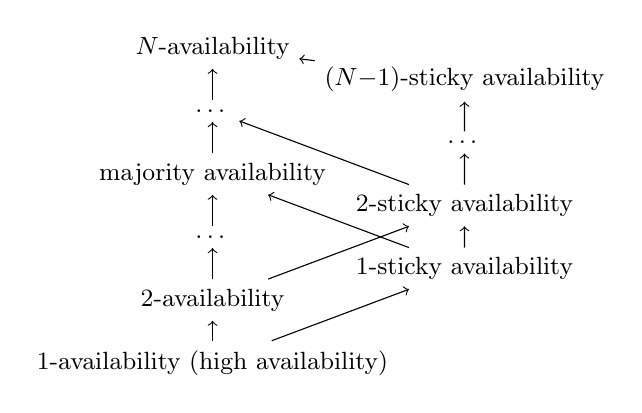
\begin{tikzpicture}[scale=0.8]
  \tikzstyle{every node}=[font=\small]
 \node[draw=none,fill=none] (1) at (0,0) {$1$-availability (high availability)}; 
 \node[draw=none,fill=none] (2) at (0,1) {$2$-availability}; 
 \node[draw=none,fill=none] (m-1) at (0, 2) {\ldots}; 
 \node[draw=none,fill=none] (m) at (0, 3) {majority availability}; 
 \node[draw=none,fill=none] (m+1) at (0, 4) {\ldots}; 
 \node[draw=none,fill=none] (n) at (0, 5) {$N$-availability}; 
 \node[draw=none,fill=none] (1s) at (4, 1.5) {$1$-sticky availability};
 \node[draw=none,fill=none] (2s) at (4, 2.5) {$2$-sticky availability};
 \node[draw=none,fill=none] (n2s) at (4, 3.5) {\ldots};
 \node[draw=none,fill=none] (n1s) at (4, 4.5) {$(N$$-$$1)$-sticky availability};

 \draw [->] (1) -- (2);
 \draw [->] (2) -- (m-1);
 \draw [->] (m-1) -- (m);
 \draw [->] (m) -- (m+1);
 \draw [->] (m+1) -- (n);
 \draw [->] (1) -- (1s);
 \draw [->] (1s) -- (m);
 \draw [->] (2s) -- (m+1);
 \draw [->] (1s) -- (2s);
 \draw [->] (2) -- (2s);
 \draw [->] (2s) -- (n2s);
 \draw [->] (n2s) -- (n1s);
 \draw [->] (n1s) -- (n);


\end{tikzpicture}
\label{fig:availability-order}
\caption{Hierarchy of replica availability levels for $N>3$ servers.}
\end{figure}

We show the hierarchy of replica availabilty levels in
Figure~\ref{fig:availability-order}. $K$-sticky availability subsumes
$K$-availability, but $K$-sticky availability is incomparable with
$(K+1)$-availability. $N$-sticky availability is equivalent to
$N$-availability, while majority availability subsumes $1$-sticky
availability More generally, $\lceil \frac{N}{2} \rceil$$+$$K$$-$$1$
availability subsumes $K$-sticky availability. We have omitted
discussion of operation-specific availability levels (e.g.,
$N$-availability for writes and $1$-availability for reads in a
write-all, read-one data store), system membership changes, or
heterogeneous replicas (e.g., servers in a local and remote
datacenters) but believe there are several avenues for further
taxnomization.

\subsection{Transactional Availability}

Thus far, we have focused on single-operation availability. This is
standard in distributed systems literature (e.g., atomic, regular, and
safe register models all concern single objects~\cite{herlihy-art}),
yet the database literature largely focuses on transactions: groups of
multiple operations over multiple objects. Accordingly, by itself,
replica availability is insufficient to describe availability
guarantees for transactions. Additionally, given the choice of
\textit{commit} and \textit{abort} responses---which signal
transaction success or failure to a client---we must be careful in
defining availability.

If a client wishes to execute a transaction that performs operations
on multiple data items, then the client must be able to contact and
receive a response from at least one server responsible for each data
item. This may result in lower availability than a non-transactional
requirement. Additionally, given the possiblity of aborts, we need to
ensure useful forward progress. A system can trivially guarantee
clients a response by always aborting their
transactions~\cite{transaction-liveness}. However, this is an
unsatisfactory system because nothing good (transaction commit) ever
happens; instead, we require a \textit{liveness} property. We cannot
guarantee that every transaction will commit---transactions may choose
to abort themselves---but we need to make sure that the system will
not indefinitely abort transactions on its own volition. We call a
transaction abort due to a transaction's own choosing (e.g., as part
of the transaction itself or due to a would-be integrity constraint
violation) an \textit{internal abort} and an abort due to system
implementation an \textit{external abort}.

We say that a system provides \textit{transactional availability} if,
given replica availability for every data item in a transaction, the
transaction eventually commits or internally aborts. For example,
system will violate transactional $2$-availability if client that can
contact two servers for each of data items in its transaction does not
eventually commit in the absence of internal aborts.




\section{Highly Available Transactions}
\label{sec:hats}

\begin{quote}
``...one should not throw out the C so quickly, since there are real
  error scenarios where CAP does not apply and it seems like a bad
  tradeoff in many of the other situations.''---Michael
  Stonebraker~\cite{stonebraker2010errors}
\end{quote}

HAT systems offer substantial latency and availability benefits, yet
they come with a cost. In the distributed systems community, there is
a host of results that taxonomize the relationships between various
distributed consistency models. Perhaps most famously, Brewer's CAP
Theorem---as formally proven by Gilbert and
Lynch~\cite{needed}---states that it is impossible to maintain
linearizability (``C,'' or ``consistency''---albeit poorly named), or
the ability to read the last completed write, and replica availability
in the presence of failures~\cite{needed}. While the CAP Theorem has
has roots in decades of distributed system designs~\cite{needed}, it
has had large scale impact on the design and development of
distributed systems, particularly for Internet
services---unsurprisingly, the context in which Brewer formulated his
finding.

\subsection{ACID and Modern Databases}

While linearizability is a useful property to consider, there are
several other guarantees that are perhaps more relevant to a database
system. In particular, the database tradition of providing ACID
guarantees: atomicity, consistency, isolation, and durability are,
with few exceptions, not addressed by the distributed systems
literature. There are several factors behind this occurrence, the
least of which is that distributed systems rarely consider
multi-object guarantees, whereas ACID transactions are frequently used
to provide semantic guarantees across multiple operations on multiple
objects. While linearizability (unfortunately often called
``atomicity'') ``composes'' across multiple objects, a linearizable
system does not provide ACID ``atomicity'' (which we will call
``transactional atomicity'' for clarity): just because two writes are
visible to all writers immediately after they complete does not, on
its own, provide any guarantees about the mutual visibility of the two
writes.

Database designers and researchers have long realized that
serializability---the gold standard of ACID isolation, which
guarantees application-level consistency---is not achievable in a
highly available system. Indeed, decades of research on
semantics-based concurrency control and coordination-reducing
techniques such as escrow transactions and sagas allow serializability
in the presence of partial system knowledge or otherwise reduce
coordination cost. However, the majority of these algorithms are
intended to preserve application-level consistency, which, for
arbitrary applications and arbitrary sequence of operations, cannot be
ensured with high availability in the presence of partitions.

Of course, database systems offer a range of ACID properties besides
serializability. Even on a single-node system, the coordination
penalties associated with ensuring equivalence with a serial execution
can be severe and manifest themselves in the form of concurrency
control contention (and, subsequently, performance degradation,
scalability limitations, and, often, external aborts like
deadlocks). Instead, databases offer a host of so-called \textit{weak
  isolation} models that allow varying restrictions on the space of
schedules that are allowable by the system. None of these weak
isolation models guarantees serializability, but the benefits of these
models can outweigh the costs of possible application-level
consistency anomalies that arise from their use.

To understand the prevalence of these weak isolation models, we
surveyed the default and maximum isolation models provided by 18
relational databases, often claiming to provide ``ACID'' or ``NewSQL''
functionality. As shown in Table~\ref{table:existing}, only three out
of 18 databases provides serializability by default, and at least
eight do not provide serializability as an option at all. This is
particularly surprising when we consider the widespread deployment of
many of these databases, like Oracle 11g, which are known to power
major businesses and product functionality. We might view the use of
weak consistency is somewhat of an ``arms race'': anecdotally, one
major RDBMS vendor was forced to lower their default isolation level
in order to compare favorably in out-of-the-box performance
comparisons with its major competitor, which had already lowered its
default setting. Applications can guard against inconsistency in a
weakly isolated environment by performing their own locking external
to the database or by performing ad-hoc concurrency control within the
database. However, this appears error-prone and, without further
evidence, it remains somewhat puzzling why this is indeed favorable to
providing serializability with in the database itself.

\begin{table}
\begin{small}
\begin{tabular}{|l|c|c|}
\hline
Database & Default & Maximum\\\hline
Actian Ingres 10.0/10S~\cite{actian-docs} & S & S\\
Aerospike~\cite{aerospike-docs} & RC & RC\\
Akiban Persistit~\cite{akiban-docs} & SI & SI\\
Clustrix CLX 4100~\cite{clustrix-docs} & RR & ?\\
Greenplum 4.1~\cite{greenplum-docs} & RC & S \\
IBM DB2 10 for z/OS~\cite{db2-docs} & CS & S\\
IBM Informix 11.50~\cite{informix-docs} & Depends & RR\\
MySQL 5.6~\cite{innodb-docs} & RR & S \\
MemSQL 1b~\cite{memsql-docs} & RC & RC\\
MS SQL Server 2012~\cite{ms-sql-docs} & RC & S \\
NuoDB~\cite{nuodb-docs} & CR & CR\\
Oracle 11g~\cite{oracle-docs} & RC & SI\\
Oracle Berkeley DB~\cite{bdb-reg-docs} & S & S\\
Oracle Berkeley DB JE~\cite{bdb-je-docs} & RR & S\\
Postgres 9.2.2~\cite{postgres-docs} & RC & S\\
SAP HANA~\cite{hana-docs} & RC & SI\\
ScaleDB 1.02~\cite{scaledb-docs} & RC & RC\\
VoltDB~\cite{voltdb-docs} & S & S\\
\hline
\multicolumn{3}{|p{7cm}|}{{\footnotesize RC: read committed, RR: repeatable read, SI: snapshot isolation, S: serializability, CS: cursor stability, CR: consistent read}}\\\hline

\end{tabular}
\caption{Default and maximum isolation levels for ACID and NewSQL
  databases as of January 2013 (from
  \protect\cite{needed-hotos}).}\vspace{-1.5em}
\label{table:existing}
\end{small}
\end{table}

Given that these transactional models are frequently used, our
inability to provide serializability to provide general-purpose HATs
appears not to be a show-stopper. If applications cope with
inconsistency or, on a single node server, have already decided that
the benefits of weak isolation outweigh potential application
inconsistencies, then perhaps, in a highly available environment, some
may make a similar decision given the appropriate choice of semantic
guarantees.

The primary challenge in providing weak isolation in a HAT context is
that, unfortunately, it is unclear \textit{which} isolation guarantees
can be provided with high availability. Standard discussions of weak
isolation are presented in a single-node context---a possible
consequence of their original context: a lock-based (and therefore
unavailable, even in a distributed context) single-server
deployment~\cite{needed}. We are not aware of any prior literature
that provides guidance as to the relationship between weak isolation
and high availability. Prior work has examined the relationship
between serializability and high availability and weak isolation on a
single-server but never weak isolation and high availability taken
together. This apparent gap in the database literature is a possible
contributing factor to the often-apparent attitude that
general-purpose transactional semantics are either too expensive or
too lacking in availability guarantees to provide in modern
distributed databases---except under special circumstances, such as
operations over groups of co-located data items.

\subsection{Achievable HAT Semantics}

In this paper, we will describe which ACID semantics are achievable in
HATs as well as which are not. Our strategy is to explore successively
more powerful models until we reach a frontier of semantic guarantees
which are unavailable to HATs. To begin, we present achievable
semantics, offering proof-of-concept algorithms to demonstrate
feasibility. When possible, we draw on existing properties and
definitions from the database and distributed systems literature,
providing a brief, informal explanation of each guarantee and
illustrate it with an example. For our ACID guarantees, we draw
largely on Adya's thesis work on defining weak isolation
models~\cite{needed} and, where appropriate, supplement with
definitions and discussion from Berenson et al.'s SIGMOD 1995 critique
of the ANSI SQL Specification~\cite{needed} (hereafter, Berenson) as
well as the ANSI SQL specification~\cite{needed} (hereafter, ANSI)
itself. For other guarantees, such as session properties, we draw on
both the database and distributed systems literature. We provide a set
of formal definitions and semantics in the Appendix.

\subsubsection{ACID Isolation Guarantees}

To begin, Adya's \textit{Read Uncommitted} isolation requires that
transactions are totally ordered and that writes within transactions
are ordered consistently with this order (prohibiting ``Dirty
Writes,'' or $G0$)~\cite{adya}. If two transactions write to the same
set of data items, then the final database state cannot contain the
``earlier'' transaction's writes to the data items. For example, in
the below example, $T_3$ should eventually only read $a=b=1$ or
$a=b=2$ but not $a=2, b=1$:
\begin{align*}
\small
T_1 &: w_x(1)~w_y(1)
\\T_2 &: w_x(2)~w_y(2)
\\T_3 &: r_x(a)~r_y(b)\\[-2em]
\end{align*}
The difference between this total order on transactions and the total
order required by serializability is that the Read Uncommitted total
order is completely arbitrary (i.e., an order must exist), whereas a
serializable total order must be equivalent to a serial
execution. Interestingly, Read Uncommitted is a close analog with
eventually consistent systems's concept of replica convergence, in
which all replicas for a data item must end up with the same data
item. This convergence is usually achieved by picking a ``winning''
update---which requires ordering---or by maintaining a growing a set
of updates---whose cardinality implicitly defines an order (with
convergence achieved when all updates are in the set); we can see Read
Uncommitted as a cross-item convergence property. It is easily
achieved via applying the same logical timestamp to each update in a
transaction.

\textit{Read Committed} isolation requires that transactions do not
read uncommitted versions of data items (prohibiting both ``Dirty
Writes''---as above---and ``Dirty Reads'' phenomena; captured by
Adya's $G1\{a,b,c\}$, ANSI's $P1$, and Berenson's ``broad'' $P1$
(2.2)). For instance, in the example below, $T_3$ should never see
$a=1$, and, if $T_2$ aborts, $T_3$ should never read $a=3$:
\vspace{-.5em}
\begin{align*}
\small
T_1 &: w_x(1)~w_x(2)
\\T_2 &: w_x(3)\\
T_3 &: r_x(a)\\[-2em]
\end{align*}
It is fairly easy to prvent ``Dirty Reads'': if transactions never
write uncommitted data to the database, then transactions will never
read dirty data. Clients can buffer their writes until they commit,
or, alternatively, can send them to servers, who will not serve writes
until clients notify that they have been committed.

\textit{Repeatable Read} isolation is a contentious property. As
Berenson et al. point out, Gray's original Repeatable Read lock-based
implementation provides substantially richer guarantees than those
that are promised by the ANSI SQL specification. Gray, Berenson, and
Adya effectively preclude all serializability anomalies but the
Phantom Problem (which we have explicitly not yet considered and will
do so in Section~\ref{sec:unachievable-hat}). Nevertheless, the ANSI
SQL specification provides a useful property which, although is not
true to Gray's spirit of Repeatable Read, is used in distributed
consistency models. The ANSI Repeatable Read guarantee requires that,
along with observing Read Committed isolation, each transaction can
only read only version of each data item that it did not itself
produce (Berenson et al. call this preventing ``Fuzzy Read,'' or
P2). In the example below, $T_3$'s must see $a=1$:
\begin{align*}
\small
T_1 &: w_x(1)
\\T_2 &: w_x(2)
\\T_3 &: r_x(1)~r_x(a)
\end{align*}
This isolation property is much weaker than serializability, but it is
a good faith literal interpretation of the phrase ``Repeatable Read'':
transactions see their own writes. By itself, this property can be
implemented trivially---always read \texttt{null} for each
key. However, when coupled with additional properties, like
transactional atomicity, it becomes stronger: the repeated reads must
also obey some additional ordering properties. Distributed systems
describe a ``consistent snapshot'' across a set of related events as a
\textit{cut} across a set of participants or, in our case, data
items. Accordingly, to capture the notion that the transaction should
read from a consistent cut, and to disambiguate from the
aforementioned stronger Repeatable Read properties, we call ANSI SQL
Repeatable Read \textbf{Cut Isolation}. In the absence of additional
guarantees, it is possible to satisfy cut isolation with high
availability by caching each transaction's reads or, alternatively,
using multi-versioning on the server and ensuring that each
transaction's successive reads return the same version of each data
item.

We can consider two variants of Cut Isolation. The first is relatively
straightforward, and reasons about cuts over discrete data items. We
will call this \textit{Item Cut Isolation}. The second is known as
preventing the \textit{Phantom Problem}, whereby two successive
predicate-based reads return different data. We call predicate-based
cut isolation, which prevents Phansoms, \textbf{Phantom Cut
  Isolation}.\footnote{Oracle provides an isolation level called
  ``Statement Level Read Consistency''; this is analogous to Phantom
  Cut Isolation at the level of a single statement. We do not consider
  this isolation model here as it is subsumed by standard Snapshot
  Isolation but we believe it is easily adaptable.}

\subsubsection{ACID Atomicity Guarantees}

Transactional atomicity is core to ACID guarantees. Although, at least
by the acronym, not an ``isolation'' property, transactional atomicity
restricts transactions' ability to view the effects of partially
completed transactions: within a transactions, either all effects of
another transaction are observed, or none are (equivalently, once some
of the effects of a transaction are observed, all effects are
observed). This is a strictly stronger guarantee than Read Committed
isolation because, in Read Committed, we can read a subset of
committed writes whereas, with Transactional Atomicity, we must read
all of them. For example, if $T_1$ commits, then, given Transactional
Atomicity, $T_2$ must observe $b=c=1$ (or later versions):
\vspace{-.5em}
\begin{align*}
\small
T_1 &: w_x(1)~w_y(1)~w_z(1)
\\T_2 &: r_x(a)~r_y(1)~r_x(b)~r_z(c)~\\[-1.5em]
\end{align*}
$T_2$ can also observe $a=\bot$ or $a=1$.

Perhaps perplexingly, discussions of Transactional Atomicity are
absent from existing discussions of weak isolation levels. This is
perhaps again due to the single-node context in which prior work was
developed: on a single server, atomicity is near-trivial to achieve
via lightweight locking and/or local concurrency control over data
items. (In this spirit, multi-item atomicity is common in so-called
``entity groups,'' which logically represent groups of co-located
items.) In contrast, in a distributed environment, atomicity over
arbitrary groups of items is considerably more difficult to achieve
with high availability. The key challenge is that different servers
responsible for subsets of a transaction's updates must coordinate
regarding when to reveal their writes to a transaction---without
violating availability due to, say, locking, or a missing
transactional write.

Together with Cut Isolation, Transactional Atomicity prevents Read
Skew (Berenson et al.'s A5A).

(MORE HERE FROM MY NOTES)

Transactional atomicity is achievable in a HAT environment. To ensure
transactional atomicity, servers only need to know when all of a
transaction's updates are present on their respective servers but do
not need to know when all respective servers know when all of a
transaction's updates are present on their respective servers. This
subtle distinction corresponds to the difference between the
distributed systems concepts of consensus and uniform reliable
broadcast. The former requires explicit agreement across servers,
while the latter simply requires that, if one server reveals a write,
then all servers reveal the write.

(TODO: fix me--HotOS copy!)

Nonetheless, Coordinating transactional atomicity across replicas is
challenging. For example, if, as is common~\cite{readonly, eiger}, we
use a master to determine the correct set of updates to read, then the
system will not be available when clients are partitioned from the
master. Instead, we rely on decentralized \textit{background}
agreement to decide when to show new values, which can safely stall in
the presence of partitions. Each server keeps a known good value for
each data item $d$ it is assigned, $d_{good}$ and a set of pending
updates to $d$, $d_{pending}$. We use asynchronous agreement to move
updates from $d_{pending}$ to $d_{good}$: all of $d_{good}$'s
transactional siblings (or later values) are guaranteed present on all
replicas. Without aborts, this requires only one synchronous round
trip time (RTT).

\noindent\textit{Writes:} First, consider the case where transactions
do not internally abort. On commit, for each written data item $d$, we
send the last written value of $d$ ($d_v$) with the transaction ID and
$L_v$, a list of all data items and values written in the transaction,
to available replicas for $d$. The replicas immediately reply with a
response to \textit{commit}, place $d_v$ it in their respective
$d_{pending}$, and send a receipt to all replicas for items in
$L_v$. Once a server receives receipts from all replicas for all items
in $L_v$, the server sets $d_{good} = d_v$ if $d_v$'s ID is greater
than $d_{good}$'s ID. Accordingly, a new value will only appear in
$d_{good}$ when the other values written with $d_{good}$ ($L_v$) are
resident on every respective replica (though possibly in their
$d_{pending}$).\vspace{.5em}

\noindent\textit{Reads:} Each client maintains a vector of transaction
IDs $V$, with one entry per data item ($V(d)$). When a client reads a
new data item $d_i$, the server returns both $d_i$ and $L_v$, and, for
all data items $k \in L_v$, the client sets $V(k)$ to $d_i$'s ID. When
a client sends a read request for item $x$, it also sends $V(x)$, and
the replica returns \textit{either} $x_{good}$ if it matches $V(x)$ or
occurs after $V(x)$ in the transaction order or, if $x_{good}$ is
unsatisfactory, $V(x)$ from $x_{pending}$. If $V(x)$ is empty, the
server returns $x_{good}$.\vspace{.5em}

\noindent\textit{Aborts:} If we allow internal aborts, writes require
2 RTTs: one to check constraints and one to execute the above. Write
propagation and update visibility are achieved asynchronously, as in
the no-abort case.\vspace{.5em}

This implementation is entirely masterless and both reads and writes
do not block for coordination. One key property is that we do not, in general,
dictate when writes become visible (see: session guarantees,
\S\ref{sec:impossible}). Accordingly, it is highly available.\vspace{.5em}

\subsubsection{Session Guarantees}

So far, our models have not considered guarantees across transactions,
but, in the distributed systems context, many useful \textit{safety}
guarantees span multiple operations. There is no guarantee of forward
progression between transactions or any guarantees on the ordering
between transactions (other than that there exists some arbitrary
ordering).

\textit{Session guarantees} are used to describe continuity between
groups of transactions. Informally, a \textit{session} is a form of
context that consists of logical state that should persist between
operations. Users accessing a web site may want to experience a notion
of ``forward progress'' for the duration that they are logged in, and
the duration of the ``log in'' to ``log out'' period forms a
session. We can define session guarantees at several granularities
(e.g., per-transaction, per-client, per-hour) but we choose to operate
under a client-centric model.

There are several guarantees that we can make with high availability:

\vspace{.25em}\noindent\textit{\textbf{Monotonic reads}} stipulates
that a client's subsequent reads to a given object ``never return any
previous values''; reads from each item progress forward in a total
order. Under Read Uncommitted, the ordering of reads should respect the
total ordering on transactions.

\vspace{.25em}\noindent\textit{\textbf{Monotonic writes}} requires
that transactions from each individual client be serialized. Under
Read Uncommitted, the transaction order should also respect the order
in which each client submitted transactions.

\vspace{.25em}\noindent\textit{\textbf{Writes Follow Reads}} requires
that, if a client reads a write originating from transaction $T_1$
then performs transaction $T_2$, then a client can only read $T_2$'s
writes if it can also read $T_1$'s prior write (or overwritten values
for $T_1$'s write). This requirement forms the basis for potential
causality: writes follow reads obeys the ``reads-from'' relation that
captures all events that influenced each
transaction~\cite{causalmemory}. Under Read Uncommitted, the
transaction order should respect the reads-from order (note that the
total order on transactions precludes reads-from cycles).

We can achieve the above guarantees by forcing servers to wait to
reveal new writes until their respect dependencies are fulfilled on
all replicas. In the case of Monotonic Reads, servers should only
reveal new writes to a data item when all other servers responsible
for the item have also seen them. Otherwise, a client might read a
newer version, subsequently become partitioned from its prior server,
and contact a comparatively out-of-date server. In the case of
Monotonic Writes, each new write should become visible only when each
client's prior write is visible everywhere, along with Monotonic Reads
guarantees. For Writes Follow Reads, a servers should similarly wait
to reveal items until their dependencies are present
everywhere.

Effectively, this mechanism requires that clients only read from a
globally agreed upon lower bound on the writes in the system. This is
indeed highly available as a client will never block due to inability
to find a server with a sufficiently up-to-date version of a data
item. However, it does not imply that transactions will read their own
writes or provide much confidence in making forward progress through
the version history in the presence of partitions. The problem is
that, if a server is partitioned, under the highly available model, we
cannot discount the possibility that an unfortunate client will be
forced to issue her next requests against the partitioned server!

The solution to this conundrum is to give up high availability in
favor of sticky availability. Sticky availability permits two
additional models, which we first define and then prove are
unachievable in a generic highly available system:

\noindent\textit{\textbf{Read your writes}} requires
that whenever a client reads a given data item after updating it, the
read returns the updated value (or a value with a higher ID).

\vspace{.25em}\noindent\textit{\textbf{Causal consistency}} is the
combination of all of the prior session
guarantees~\cite{daudjee-session} and is also referred to as PL-2L
isolation~\cite{adya}). We can also consider arbitrary
application-defined partial orders, as in explicit
causality~\cite{explicit-socc}, if dependencies are specified at
commit time.

Read your writes is unavailable in a highly available system. Consider
a client that executes the following two transactions in succession:
\vspace{-.5em}
\begin{align*}
\small
T_1 &: w_x(1)
\\T_2 &: r_x(a)
\end{align*}
If the client executes $T_1$ against a server that is partitioned from
the rest of the other servers, the server must allow $T_1$ to
commit. If the client executes $T_2$ against the same (partitioned)
server, then it will be able to read its writes. However, if the
network topology shifts and the client can only contact a different
server which is partitioned from the rest of the cluster, then the
client will not be able to read its own writes and the system will
have to either stall indefinitely to allow the client to read her
writes (violating transactional availability) or will have to
sacrifice read your writes. Accordingly, read your writes requires
stickiness, and, because causal consistency requires read your writes,
causal consistency also requires stickiness.

Read-your-writes can be accomplished via client-side caching and
alternatively comes ``for free'' when requests are routed to a sticky
set of servers. Achieving causal consistency requires maintaining
read-your-writes along with the prior session guarantees. Both are
reasonable strategies often employed in real-world
systems~\cite{vogels-defs}, albeit at the cost of true high
availability or client-side storage. Perhaps interestingly,  

We discuss additional uses for stickiness in Section~\ref{sec:discussion}.

\subsubsection{Additional Guarantees}

A HAT system can make \textbf{limited consistency} guarantees. It can
execute commutative and logically monotonic~\cite{needed} operations
without the risk of invalidating (also monotonic) application-level
integrity constraints. Our goal in this paper is not to sketch the
entire space of consistency models that are achievable (see
Section~\ref{sec:futurework}, however we specifically evaluate TPC-C
transaction semantics under HAT consistency guarantees in
Section~\ref{sec:Evaluation}.

As we briefly discussed in Section~\ref{sec:availabile}, a client
requiring \textbf{durability} of surviving $F$ server faults requires
at least $F+1$-availability.

Finally, to require that servers propagate writes between replicas, we
can require \textbf{convergence}, or eventual consistency for each
data item: in the absence of new mutations to a data item, in the
absence of partitions, all servers eventually agree on the value for
each item. This is typically accomplished by any number of
anti-entropy protocols, which periodically update neighboring servers
with the latest value for each data item. This convergence property
should be considered mandatory given the spirit of existing literature
on isolation protocols: in all models we have encountered, the
database should behave as if there is some total order over
transactions. Indeed, non-convergent systems are remarkably difficult
to reason about.

\subsection{Unachievable HAT Semantics}
\label{sec:unachievable-hat}

While there are infinitely many HAT models
(Section~\ref{sec:futurework}), at this point, we have exhausted our
range of achievable, previously defined (useful) HAT semantics. Before
summarizing our possibility results, we will present impossibility
results for HATs, also defined in terms of previously identified
isolation and consistency anomalies.

\subsubsection{Unachievable ACID Isolation}

The simplest way to describe which isolation properties are achievable
with high availability is in terms of preventing different isolation
anomalies. We have already shown that it is possible prevent several
anomalies, like Dirty Read, Dirty Write, Fuzzy Read, and atomicity
violations. In this section, we demonstrate that preventing Lost
Update, Write Skew, and Phantoms requires unavailability.

In the words of Berenson et al., \textbf{Lost Update} occurs when one
transaction $T1$ reads a given data item, a second transaction $T2$
updates the same data item, then $T1$ modifies the data item based on
its original read of the data item, ``missing'' or ``losing'' $T2$'s
newer update. Consider the following transactions:
\begin{align*}
\small
T_1 &: r_x(a) w_x(a+1)
\\T_2 &: w_x(2)
\end{align*}
If $T_1$'s read from $x$ precedes $T_2$'s write to $x$ but $T_2$'s
write to $x$ precedes $T_1$'s write to $x$, then a database containing
only these two transactions will end in a state that could not have
resulted in a serial execution.

It is impossible to prevent Lost Update in a highly available
environment. Consider two clients who submit the following $T_1$ and
$T_2$ on opposite sides of a network partition:
\begin{align*}
\small
T_1 &: r_x(100)~w_x(100+20=120)
\\T_2 &: r_x(100)~w_x(100+30=130)
\end{align*}
The final state of the database will converge to an execution that
could not have resulted from a serial excecution. To prevent this from
happening, either $T_1$ or $T_2$ should not have committed. Each
client's respective server might try to detect that another write
occurred, but this requires knowing the version of the latest write to
$x$. In this example, this reduces to a requirement for
linearizability, which is, via Gilbert and Lynch's proof of the CAP
Theorem, provably unachievable with high availabilty.

\textbf{Write Skew} is a generalization of Lost Update to multiple
keys. It occurs when one transaction $T1$ reads a given data item $x$,
a second transaction $T2$ reads a different data item $y$, then $T1$
writes to $y$ and commits and $T2$ writes to $x$ and commits. As an
example of Write Skew, consider the following two transactions:
\begin{align*}
\small
T_1 &: r_y(0)~w_x(1)
\\T_2 &: r_x(0)~w_y(1)
\end{align*}
As Berenson et al. describe, if there was an integrity constraint
between $x$ and $y$ such that only one of $x$ or $y$ should be one at
any given time, then this write skew would lead to a non-serializable
execution. Write skew in particular is a somewhat esoteric
anomaly---for example, it does not appear in TPC-C---but, as a
generalization of Lost Update, is also unavailable.

The inability to prevent Lost Update means that Consistent Read,
Snapshot Isolation, and Cursor Stability are all unavailable. The
inability to prevent Lost Update or Write Skew means that Repeatable
Read, Conflict Serializability, and One-Copy Serializability are
unavailable.

\subsubsection{Unavailable Recency Guarantees}

Data storage engines make various recency guarantees on reads of data
items. One of the most famous is linearizability, which states that
reads will return the last completed write to a data item, and there
are several other (weaker) variants such as safe and regular register
semantics. When applied to transactional semantics, the combination of
one-copy serializability and linearizability is called \textit{strong
  (or strict) one-copy serializability} or \textit{externally
  consistent transactions} (e.g., Spanner). It is also common,
particularly in systems that allow reading from masters and slaves, to
provide a guarantee such as ``read a version that is no more than five
seconds out of date'' or similar. Unfortunately, as the CAP Theorem
demonstrates, linearizability is unavailabile, and any indefinitely
long partition can cause violation of any recency bound.

\subsection{Summary}
\label{sec:hat-summary}

We summarize our results in Table~\ref{table:hatcompared}. A wide
range of isolation levels are achievable in a highly available system,
including transactional atomicity, cut isolation, and several session
guarantees. With sticky availability, a system can achieve PRAM
consistency, read your writes guarantees, and causal
consistency. However, many other prominent models, such as Snapshot
Isolation, One-Copy Serializability, and Strict Serializability cannot
be achieved due to the inability to prevent Lost Update and Write Skew phenomena.

We illustrate the hierarchy of available, sticky available, and
unavailble consistency models we have discussed in
Table~\ref{fig:hatcompared}. Many models are simultaneously
achievable: for example, a HAT system can provide monotonic reads and
transactional atomicity or transactional atomicity and read your
writes and, for maximum semantic richness, can provide all of
Transactional Atomicity, Predicate Cut Isolation, Monotonic Reads,
Monotonic Writes, and Writes Follow Reads. An unavailable system might
provide PRAM and Serializability, as advocated by Salem and
Daudjee~\cite{needed}.

To the best of our knowledge, this is the first unification of
database ACID, distributed consistency, and session guarantee
models. Perhaps satisfactorily, strong one-copy serializability
subsumes all other models, while considering the (large) power set of
all compatible models (e.g., only considering client-centric session
consistency guarantees, the diagram depicts 32 possible HAT
combinations) hints at the vast expanse of consistency models found in
the literature. This taxonimization is \textit{not} exhaustive, but we
believe it lends substantial clarity into the relationships between a
large subset of the prominent ACID and distributed consistency
moels. Additional models of read/write transactions that we have
omitted should be easily classifiable based on the available
primitives and unavailable anomalies we have already discussed.

 \newcommand{\lostupdate}{$^\dagger$}
 \newcommand{\rwskew}{$^\ddagger$}
 \newcommand{\linearizable}{$^\oplus$}

\begin{table}
\begin{tabular}{| c | p{6cm} | }\hline
HA & Transactional Atomicity (TA), Read Uncommitted (RU), Read
Committed (RC), Item Cut Isolation (P-CI), Predicate Cut Isolation
(P-CI), Monotonic Reads (MR), Monotonic Writes (MW), Writes Follow
Reads (WFR)\\\hline Sticky-HA & Read Your Writes (RYW), PRAM,
Causal\\\hline Unavailable & Cursor Stability (CS)\lostupdate,
Snapshot Isolation (SI)\lostupdate, Repeatable Read
(RR)\lostupdate\rwskew, Conflict Serializability
(CSR)\lostupdate\rwskew, One-Copy Serializability
(1SR)\lostupdate\rwskew, Recency\linearizable, Safe\linearizable,
Regular\linearizable, Strong 1SR\lostupdate\rwskew\linearizable
\\\hline
\end{tabular}
\caption{Summary of highly available, sticky highly available, and
  unavailable models considered in this paper. Unavailable models are
  labeled by cause of unavailability: preventing lost
  update\lostupdate, preventing write skew\rwskew, and requiring
  recency guarantees\linearizable.}
\label{table:hatcompared}
\end{table}

\begin{figure}
\centering
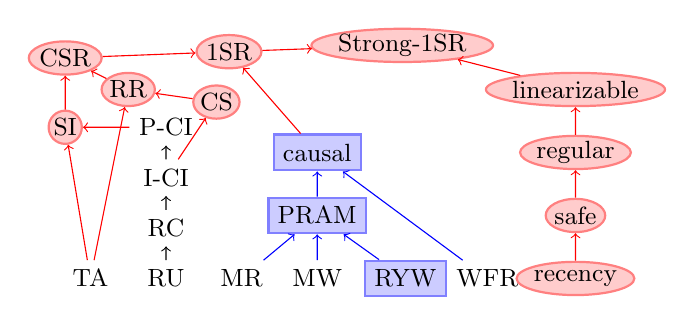
\begin{tikzpicture}[scale=0.8]
  \tikzstyle{sticky}=[rectangle,draw=blue!50,fill=blue!20,thick]
  \tikzstyle{noha}=[ellipse,draw=red!50,fill=red!20,thick, inner sep=0pt,minimum size=12pt]

  \tikzstyle{every node}=[font=\small]



 \node[draw=none,fill=none] (ici) at (1.2, 1.6) {I-CI};
 \node[draw=none,fill=none] (pci) at (1.2, 2.4) {P-CI};
 \node[draw=none,fill=none] (rc) at (1.2, .8) {RC};
 \node[draw=none,fill=none] (ru) at (1.2, 0) {RU};

 \node[draw=none,fill=none] (ta) at (0, 0) {TA};
 \node[draw=none,fill=none] (mr) at (2.4, 0) {MR};
 \node[draw=none,fill=none] (mw) at (3.6, 0) {MW};
 \node[draw=none,fill=none] (wfr) at (6.3,0) {WFR};
 \node at (5,0) [sticky] (ryw) {RYW};

 \node[noha](recency) at (7.7, 0) {recency};
 \node[noha](safe) at (7.7, 1) {safe};
 \node[noha](regular) at (7.7, 2) {regular};
 \node[noha](linearizable) at (7.7, 3) {linearizable};
 \node at (3.6, 2) [sticky] (causal) {causal};
 \node at (3.6, 1) [sticky] (pram) {PRAM};
 \node[noha] (cs) at (2, 2.8) {CS};
 \node[noha] (rr) at (.6, 3.0) {RR};
 \node[noha] (si) at (-.4, 2.4) {SI};
 \node[noha] (s) at (-.4, 3.5) {CSR};
 \node[noha] (sr) at (2.2, 3.6) {1SR};
 \node[noha] (ssr) at (4.95, 3.7) {Strong-1SR};

 \draw [->, red] (recency) -- (safe);
 \draw [->, red] (safe) -- (regular);
 \draw [->, red] (regular) -- (linearizable);
 \draw [->, red] (linearizable) -- (ssr);
 \draw [->, red] (sr) -- (ssr);
 
 \draw [->] (ru) -- (rc);
 \draw [->] (rc) -- (ici);
 \draw [->] (ici) -- (pci);

 \draw [->, blue] (mr) -- (pram);
 \draw [->, blue] (mw) -- (pram);
 \draw [->, blue] (wfr) -- (causal);
 \draw [->, blue] (ryw) -- (pram);
 \draw [->, blue] (pram) -- (causal);

 %\draw[snake=coil, segment aspect=0, segment amplitude=.75pt, segment length=2pt] (ru) -- (mr);
 %\draw[snake=coil, segment aspect=0, segment amplitude=.75pt, segment length=2pt] (rc) -- (ta);
 %\draw[snake=coil, segment aspect=0, segment amplitude=.75pt, segment length=2pt] (ici) -- (ta);
 %\draw[snake=coil, segment aspect=0, segment amplitude=.75pt, segment length=2pt] (pci) -- (ta);
 %\draw[snake=coil, segment aspect=0, segment amplitude=.75pt, segment length=2pt] (rc) -- (mr);
 %\draw[snake=coil, segment aspect=0, segment amplitude=.75pt, segment length=2pt] (pci) -- (mr);
 %\draw[snake=coil, segment aspect=0, segment amplitude=.75pt, segment length=2pt] (ici) -- (mr);
 %\draw[snake=coil, segment aspect=0, segment amplitude=.75pt, segment length=2pt] (ta) -- (ru);
 %\draw[snake=coil, blue, segment aspect=0, segment amplitude=.75pt, segment length=2pt] (ru) -- (causal);
 %\draw[snake=coil, segment aspect=0, segment amplitude=.75pt, segment length=2pt] (mr) -- (mw);
 %\draw[snake=coil, segment aspect=0, segment amplitude=.75pt, segment length=2pt] (wfr) -- (mw);
 %\draw[snake=coil, blue, segment aspect=0, segment amplitude=.75pt, segment length=2pt] (wfr) -- (ryw);

 \draw [->, red] (ici) -- (cs);
 \draw [->, red] (cs) -- (rr);
 \draw [->, red] (pci) -- (si);
 \draw [->, red] (rr) -- (s);
 \draw [->, red] (si) -- (s);
 \draw [->, red] (ta) -- (si);
 \draw [->, red] (ta) -- (rr);
 \draw [->, red] (s) -- (sr);
 \draw [->, red] (causal) -- (sr);

\end{tikzpicture}
\label{fig:hat-order}
\caption{HAT, sticky HAT (in boxes), and unavailable models (circled)
  from Table~\protect\ref{table:hatcompared} compared
  graphically. Directed edges represent ordering by model
  strength. Models that do not share a common ancestor can be
  simultaneously achieved, and the resulting availability is that of
  the weakest available model in the combination.}
\label{fig:hatcompared}
\end{figure}


\subsection{Discussion}
\label{sec:discussion}

In this section, we discuss several subleties we have mostly elided up
to this point, specifically addressing model composition,
transactional atomicity versus linearizability, and stickiness
requirements.

\noindent\textbf{Model Composition} may be non-trivial. Consider the following transactions:
\begin{align*}
\small
T_1 &: w_x(1)~w_y(1)
\\T_2 &: w_x(2)~w_y(1)
\\T_3 &: r_x(a)~r_y(b)
\end{align*}
If we want to guarantee both cut isolation and transactional atomicity
and these are the only transactions that are executed by the system,
then $T_3$ needs to read $a=b=\bot$, $a=b=1$, or $a=b=2$. This means
that either the implementation should frequently return null
(definitely undesirable and possibly non-convergent), keep multiple
versions of each data item (necessitating potentially complicated
distributed garbage collection), or use pre-declared read sets to
fetch a consistent cut of keys before the transaction begins to
execute. Using client-side caching can alleviate some of these
challenges, but then the system becomes sticky high available.

Composition cost varies by property. For instance, Charron-Bost has
proven that, to capture causality between $N$ communicating processes,
standard vector-based approaches face an upper bound of $O(N)$. This
means that, with $100,000$ clients, each write might be accompanied by
$100,000$ vector timestamps. This is difficult to scale. By
compromising on availability (e.g., treating a datacenter as a
linearizable cluster), this overhead can be reduced, but it is much
cheaper to provide, say, read your writes, compared to causality.

\noindent The relationship between \textbf{Transactional Atomicity and
  Linearizability} is not immediately clear. One might attempt to find
a mapping between the two: Transactional Atomicity dictates that
writes to multiple keys across multiple servers are made visible to
readers all at once, while Linearizability dictates taht writes to a
single key on multiple servers are made visible to all readers at
once. The difference is two-old. First, in linearizable (and safe and
regular) systems, writes are made visible to all clients immediately
after they finish. With Transactional Atomicity, there is no recency
requirement. Second, in linearizabile systems, all clients see all
writes at the same time. With Transactional Atommicity, clients see
writes at different times depending on which relicas they contact. We
are not aware of a comparable analog in the distributed systems
literature. Accordingly, despite apparent similarities, Transactional
Atomicity is much weaker than Linearizability.

\noindent There is a substantial \textbf{visibility benefit to sticky
  availability}: writes can safely become visible to readers much more
quickly in a sticky available system. In the model we discussed, it is
possible to achieve several properties like monotonic reads in a
highly available system by waiting until all servers have seen a
write. However, this leads to horrible visibility---new writes will
not become visible to clients in the presence of partitions. A client
that does not want to guarantee read-your-writes (due to the sticky
availability requirement) may still wish to read other clients' writes
with timeliness. Accordingly, a system may forgo high availability in
order to provide better visibility. Alternatively, a system may
enforce stickiness in the absence of partitions, then ``lose'' session
guarantees by having clients reconnect to an available replica. This
latter strategy provides session guarantees between partitions, and
each partition event may cause a ``regression'' in the desired order
of partitions, albeit at the benefit of availablilty.

It is increasingly common in the practically-oriented distributed
systems literature to assume that clients will be able to remain
sticky with servers within its datacenter. More generally, if
client-server sticky pairs are partitioned into disjoint sets, or
groups, then additional guarantees like transactional atomicity can be
accomplished with better visibility: writes can be made visible once
they are present on all other servers within a group (as opposed to
all servers in the system).





\section{evaluation}

V. Evaluation (1.5pg)

The goal in this section is twofold:
1.) Look at existing algorithms and their coordination cost in the abstract
2.) Perform limited real-world deployments to validate these abstract costs

1.) There are a bunch of existing systems that aren't HATS but provide stronger semantics. What's their cost? (N.B. this is almost a related work survey here, but I think, if done right, it can be very instructive.)
Not HA, Serializable:
* Two-phase locking: for transaction size T, T+1 round-trips (directly to each database)
* Deterministic transaction scheduling: 1 round-trip per partition (to scheduler)
* Optimistic concurrency control: 1 round-trip per partition (to database cycle checker)
* MVCC: min 1 round-trip per partition (to partition timestamp manager)

Not HA, not serializable, but "transactional":
* MDCC: need to check, 1-2 round-trip times because uses Paxos variant
* Walter: 1 rount-trip time to each preferred site
* Eiger: Sticky-HA, assumes linearizable clusters, reads/writes stall in presence of coordinator failures
* Chan and Gray read-only transaction: reads stall in the presence of coordinator failure
* Bolt-on causal consistency: sticky-HA, could be used to implement TA+RR, uses client cache
* COPS: Sticky-HA, assumes linearizable clusters
* Bayou: not HA since client doesn't cache (pretty sure)

2.) We ran YCSB on EC2 (and maybe TPC-C if we have time) with a few models:
	- Eventual Consistency
	- Eventual consistency with a "master" for updates--simulates the lower bound on a non-HAT system.
	- Transactional Atomicity and Read Committed
	
	-This is going to look a lot like the ping tests: much higher latency for "non-HATs."
	-Our Naive 2PL implementation bottlenecks extremely quickly.
	-On, say, 5 servers, can get hundreds of thousands of TPS

	-Not meant as an exhaustive study, but validates our intuitions. Coordination costs of non-HAT systems are unaccounted for, will only go up, and we haven't even talked about availability.



\section{Related Work}

There is a growing body related work on highly available semantics,
mechanisms for concurrency control, and techniques for scalable
distributed operations.

Weak consistency and high availability have been well
studied. Serializability has long been known to be
unachievable~\cite{davidson-survey} and Brewer's CAP Theorem has
attracted considerable attention~\cite{gilbert-cap}. Recent work on
PACELC expands CAP by considering connections between ``weak
consistency'' and low latency~\cite{abadi-pacelc}, while several
studies examine weak isolation guarantees~\cite{adya,
  ansicritique}. However, as we have discussed, the connection between
weak, multi-object consistency models in a distributed setting and
high availability is relatively unexplored. With the exception of our
preliminary workshop paper discussing transactional availability and
HAT RC and I-CI~\cite{hat-hotos}--- which this work expands, providing
additional algorithms and impossibility results, a full
taxonomization, and experimental and application analysis---we believe
this paper is the first to explore this area. However, several studies
rigorously classify \textit{non-HAT} semantics: Wisemann et al. have
proposed a three parameter classification for one-copy serializable
database systems, performing a more extensive classification than our
overview in Section~\ref{sec:evaluation}, including eager database
replication techniques~\cite{kemme-classification}. Additionally
several earlier surveys consider distributed mechanisms for achieving
one-copy serializability~\cite{wisemann-survey}, linearizability,
consistent snapshots, and recency bounds~\cite{ceri-mechanism,
  chen-mechanism}.

There has been a recent resurgence of interest in distributed
multi-object semantics, both in academia~\cite{kraska-s3, gstore,
  mdcc, eiger, walter,calvin, swift} and industry~\cite{orleans,
  spanner}. As discussed in Section~\ref{sec:modernacid}, classic ACID
databases provide strong semantics but their lock-based and
traditional multi-versioned implementations are unavailable in the
presence of partitions~\cite{bernstein-book, gray-isolation}. Notably,
Google's Spanner provides strong one-copy serializable
transactions. While Spanner is highly specialized for Google's
read-heavy workload, it relies on two-phase commit and two-phase
locking for read/write transactions~\cite{spanner}. As we have
discussed, the latency penalties associated with this design choice
are fundamental to serializability. For users willing to tolerate
these costs, Spanner, or similar strongly consistent, unavailable
systems---including Calvin~\cite{calvin}, G-Store~\cite{gstore},
Generalized Snapshot Isolation~\cite{generalizedsnapshot}, HBase,
HStore~\cite{hstore}, MDCC~\cite{mdcc}, Orleans~\cite{orleans},
Postgres-R~\cite{kemme-thesis}, Walter~\cite{walter}, and a range of
snapshot isolation techniques~\cite{middleware-db, kemme-snapshot,
  daudjee-snapshot}---are a reasonable choice.

With HATs, we seek an alternative set of semantics that are still
useful but do not violate requirements for high availability or low
latency. Recent systems proposals such as Swift~\cite{swift},
Eiger~\cite{eiger}, and Bolt-on Causal Consistency~\cite{bolton}
provide transactional causal consistency guarantees with varying
availability and represent a new class of sticky HAT systems.

\pbnote{add TA stuff}


% Ceri discuss distributed database update mechanisms with respect to
% linearizability, consistent snapshots (i.e., cut isolation), and
% recency bounds~\cite{ceri-mechanism}.  Chen and Pu also classify
% distributed replica maintenance from perspectives of
% linearizability,% recency guarantees, and replica
% divergence~\cite{chen-mechanism}.



%, with increasing interest in returning to transactional
%designs~\cite{spanner, walter, foundation-article, krikellas-bargain,
%  eiger}




\section{Future Work}

VII. Future Work (.75pg)

* What properties are available?
	* We've focused on ACID Isolation, but there are lots of other models to consider?
	* Which consistency criteria? Which models? There are infinite, so how do we choose?
	* Set ourselves up for APEs

* Full exploration of HAT space
	* Many parameters; $2^10$ models at the least
	* Need to mitigate the cost of tracking causality with high availability
		* The cost moving from S-HA (like Eiger) to truly HA (R-HA) seems to be high
		* e.g., Eiger relies on metadata GC to keep writes small; is O(|keys|) in limit
			* Not meant as a fault--it's optimized for a particular scenario--but curious to consider

* Revisit semantics-based concurrency control
	* Could taxonomize properties like escrow
	* Can also consider models with SLAs and bounded messaging asynchrony
	* Our focus is on "classic" distributed systems trade-off
		* However, lots of interesting hybrids (maybe cite Doug Terry's recent stuff)




\section{Conclusion}
The current state of database software offers uncomfortable and
unnecessary choices between availability and transactional semantics.
Through our analysis and experiments, we have demonstrated how goals
of high availability will remain a critical aspect of many future data
storage systems. Accordingly, we expose a broad design space of Highly
Available Transactions (HATs), which can offer the key benefits of
highly available distributed systems---''always on'' operation during
partitions and low-latency operations---while also providing a family
of transactional isolation levels and replica semantics that have been
adopted in practice.  In taxonomizing this design space, we show that
many transactional guarantees are achievable with high availability,
while a few, like preventing Lost Update and Write Skew, are not. This
offers a long-overdue connection between storage semantics studied in
the database and distributed systems communities. The subsequent
challenge is to return to issues of performance and systems
architecture within the HAT design space.  Based on our understanding
of what is desired in the field and newfound knowledge of what is
possible to achieve, we believe HATs will be an area of great
opportunity in the coming years.

%% In this paper we expose a broad design space of Highly Available Transactional 
%% Systems (HATs), which can offer the key benefits of
%% highly available distributed systems---partition tolerance and low-latency 
%% writes---while also providing a family of transactional isolation 
%% levels and replica semantics that have been widely used in practice. 
%% In taxonomizing this design space, we show that many transactional 
%% guarantees are achievable with high availability, while a few, 
%% like preventing Lost Update and Write Skew, are not. 

%% There has been some debate in the database community regarding the importance
%% of availability in modern databases; there is also concern about the utility of
%% relaxed isolation.  Our analysis and experiments in Sections~\ref{sec:motivation} 
%% and~\ref{sec:evaluation} convince us that the availability goals of the NoSQL
%% movement will remain a critical aspect of many important systems going forward, and 
%% that the isolation levels available via HATs can have significant practical impact
%% in delivering useful transactional semantics to application developers.

%% Much of the prior research in distributed transactions has focused on prototyping 
%% individual points in the design space, with a focus on providing serializability
%% at the expense of availability.  Our goal in this paper has been to take a broader view. 
%% We taxonomize the joint design space of replica consistency and transactional isolation,
%% and identify what is possible and impossible to achieve semantically via HATs.  From
%% a research perspective, this offers a long-overdue connection between storage 
%% semantics studied in the database and distributed systems communities.
%% With this understanding in hand, the next challenge is to return to issues of 
%% performance and systems architecture within the HATs design space.  Based on our 
%% understanding of what is desired in the field and what is possible to achieve, we 
%% believe this is an area of great opportunity in the coming years.



% The following two commands are all you need in the
% initial runs of your .tex file to
% produce the bibliography for the citations in your paper.
\bibliographystyle{abbrv}
% vldb_sample.bib is the name of the Bibliography in this case
\footnotesize
\bibliography{hat-vldb}  
% You must have a proper ".bib" file
%  and remember to run:
% latex bibtex latex latex
% to resolve all references

%APPENDIX is optional.
% ****************** APPENDIX **************************************
% Example of an appendix; typically would start on a new page
%pagebreak

%\begin{appendix}

%\end{appendix}

\end{document}
